% ============================================================
%  SECTION 1: TỔNG QUAN ĐỒ ÁN
% ============================================================
\chapter{Tổng quan Đồ án}

\section{Giới thiệu}

Đồ án 2 yêu cầu xây dựng một hệ thống CI/CD (Continuous Integration / Continuous Delivery)
hoàn chỉnh để triển khai, vận hành và giám sát ứng dụng microservice
\textbf{YAS — Yet Another Shop} trên nền tảng Kubernetes.

YAS là một ứng dụng thương mại điện tử mã nguồn mở được xây dựng theo kiến trúc microservice,
gồm hơn 20 service viết bằng Java/Spring Boot và Next.js. Ứng dụng sử dụng các
công nghệ hiện đại như Kafka, Elasticsearch, Keycloak, OpenTelemetry, Grafana, Loki, Prometheus và Tempo.

\subsection{Yêu cầu bắt buộc (6 điểm)}

\begin{enumerate}[label=\textbf{YC\arabic*.}]
  \item Sử dụng image có tag \texttt{main}/\texttt{latest} cho tất cả service làm mặc định.
  \item Xây dựng K8s cluster ít nhất 1 Master + 1 Worker (hoặc Minikube/K3s).
  \item \textbf{Pipeline CI:} Khi developer commit lên bất kỳ branch nào, tự động build image
        với tag = \texttt{commit\_id} và push lên Docker Hub.
  \item \textbf{Job CD \texttt{developer\_build}:} Developer chỉ định service + branch muốn test,
        pipeline deploy service đó với image mới, các service còn lại dùng \texttt{latest}.
        Cung cấp domain để developer truy cập kiểm tra.
  \item \textbf{Job CD xóa deployment} từ yêu cầu 4.
  \item \textbf{Pipeline CI/CD} tự động: (a) push \texttt{main} \textrightarrow{} deploy vào namespace \texttt{dev};
        (b) tạo tag \texttt{vX.Y.Z} \textrightarrow{} build image mới, deploy vào namespace \texttt{staging}.
\end{enumerate}

\subsection{Yêu cầu nâng cao (2+2 điểm)}

\begin{itemize}
  \item \textbf{ArgoCD (2đ):} Sử dụng ArgoCD thay thế deploy trực tiếp để quản lý GitOps
        cho môi trường \texttt{dev} và \texttt{staging}.
  \item \textbf{Service Mesh / Istio (2đ):} Cấu hình mTLS giữa các service, Authorization Policy,
        Retry Policy, và visualize topology qua Kiali.
\end{itemize}

% ============================================================
\section{Kiến trúc Hệ thống}

\subsection{Kiến trúc tổng thể}

Hệ thống được triển khai trên \textbf{K3s v1.32.5} chạy trên máy Fedora Linux 43
với cấu hình 32 CPU / 32GB RAM / 952GB NVMe. Cluster bao gồm 1 control plane node và
2 worker node.

\begin{figure}[H]
  \centering
  \IfFileExists{../yas-architecture-local.png}{
    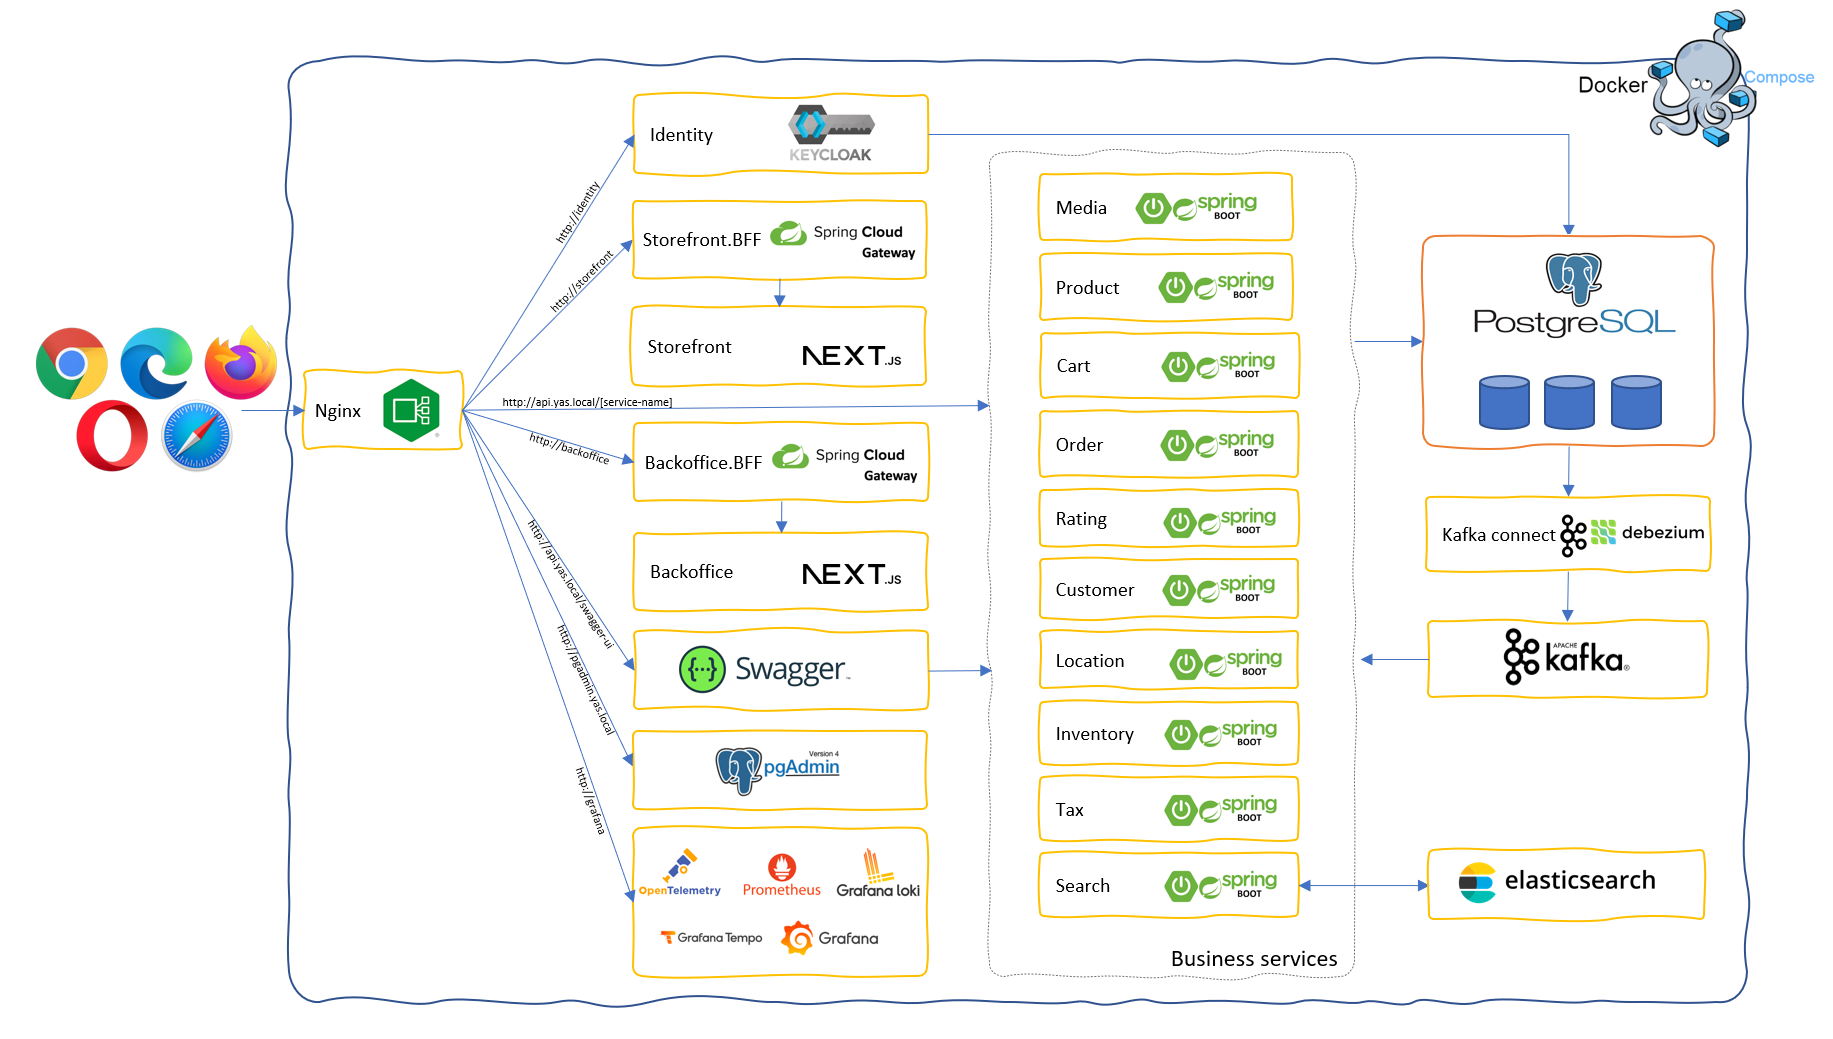
\includegraphics[width=0.9\textwidth]{../yas-architecture-local.png}
  }{
    \fbox{\parbox{0.9\textwidth}{\centering \textit{[Hình: Kiến trúc tổng thể YAS microservice]}\\\small Chèn screenshot kiến trúc hệ thống vào đây}}
  }
  \caption{Kiến trúc tổng thể YAS microservice}
  \label{fig:yas-arch}
\end{figure}

Toàn bộ hệ thống được tổ chức thành các lớp như sau:

\begin{table}[H]
  \centering
  \caption{Phân tầng hệ thống}
  \begin{tabularx}{\textwidth}{L{3cm}L{5cm}X}
    \toprule
    \textbf{Tầng} & \textbf{Namespace} & \textbf{Thành phần} \\
    \midrule
    Ingress & \texttt{ingress-nginx} & ingress-nginx-controller (LoadBalancer, klipper-lb) \\
    \midrule
    Service Mesh & \texttt{istio-system} & istiod, istio-ingressgateway, istio-egressgateway, Kiali \\
    \midrule
    Applications & \texttt{yas} & 20+ microservices (cart, order, product, customer, …) \\
    \midrule
    GitOps & \texttt{argocd} & ArgoCD server, repo-server, applicationset-controller \\
    \midrule
    Identity & \texttt{keycloak} & Keycloak 26.0.2 (OAuth2/OIDC) \\
    \midrule
    Database & \texttt{postgres} & PostgreSQL (Zalando operator), pgAdmin \\
    \midrule
    Messaging & \texttt{kafka} & Kafka 4.1.0 KRaft mode (Strimzi 0.51), AKHQ \\
    \midrule
    Search & \texttt{elasticsearch} & Elasticsearch standalone \\
    \midrule
    Cache & \texttt{redis} & Redis (session cache cho BFF) \\
    \midrule
    Observability & \texttt{observability} & Prometheus, Grafana, Loki, Tempo, OpenTelemetry \\
    \bottomrule
  \end{tabularx}
\end{table}

\subsection{Kiến trúc CI/CD Pipeline}

Pipeline CI/CD được xây dựng hoàn toàn trên \textbf{GitHub Actions}:

\begin{itemize}
  \item \textbf{CI} (\texttt{npt-ci.yml}): Chạy trên GitHub-hosted runner, không cần truy cập cluster.
  \item \textbf{CD} (các workflow deploy): Chạy trên \textbf{self-hosted runner} đặt tại máy chủ
        để có thể kết nối trực tiếp vào K3s cluster qua \texttt{127.0.0.1:6443}.
\end{itemize}

\begin{tcolorbox}[colback=gray!10, colframe=codeblue, title=Luồng CI/CD Pipeline]
  \small
  \begin{enumerate}[leftmargin=*]
    \item Developer push code lên branch bất kỳ
    \item \textbf{CI workflow} trigger: detect service thay đổi \textrightarrow{} build Maven/Docker \textrightarrow{} push image
          (\texttt{image:commit\_id}) lên Docker Hub
    \item Nếu push lên \texttt{main}: tag thêm \texttt{:latest} \textrightarrow{} trigger \textbf{Dev Deploy workflow}
          \textrightarrow{} ArgoCD sync \textrightarrow{} deploy vào namespace \texttt{dev}
    \item Nếu tạo tag \texttt{v*}: trigger \textbf{Staging Deploy workflow} \textrightarrow{} build image với tag version
          \textrightarrow{} deploy vào namespace \texttt{staging}
    \item Developer muốn test branch riêng: chạy \textbf{developer\_build} workflow thủ công
          \textrightarrow{} chỉ định service + branch \textrightarrow{} deploy vào namespace \texttt{developer}
  \end{enumerate}
\end{tcolorbox}

\subsection{Kiến trúc Service Mesh (Istio)}

Toàn bộ traffic trong namespace \texttt{yas} đi qua \textbf{Istio sidecar proxy (Envoy)},
đảm bảo mTLS STRICT giữa mọi service. Đặc biệt, \texttt{ingress-nginx} cũng được
inject sidecar và tham gia vào mesh, cho phép duy trì mTLS ngay từ điểm vào hệ thống.

% ============================================================
\section{Sơ đồ}

\subsection{Sơ đồ tổng quan Namespace và Luồng traffic}

\begin{tcolorbox}[colback=blue!3, colframe=codeblue!70, title=Luồng traffic qua K3s cluster]
  \footnotesize
  \textbf{Browser / Curl} \par
  $\downarrow$ DNS (\texttt{/etc/hosts} \textrightarrow{} \texttt{172.16.0.240}) \par
  $\downarrow$ \textbf{klipper-lb} (K3s built-in LoadBalancer, port 80/443) \par
  $\downarrow$ \textbf{ingress-nginx-controller} (namespace: \texttt{ingress-nginx}, có Istio sidecar) \par
  $\downarrow$ Istio mTLS (ISTIO\_MUTUAL via DestinationRule) \par
  $\downarrow$ \textbf{Microservice} (namespace: \texttt{yas}, pod có Envoy sidecar 2/2) \par
  $\downarrow$ Service-to-service: mTLS STRICT, Authorization Policy kiểm soát từng cặp
\end{tcolorbox}

\subsection{Sơ đồ K3s Multi-node Cluster}

\begin{table}[H]
  \centering
  \caption{Cấu hình K3s Cluster}
  \begin{tabularx}{\textwidth}{L{3cm}L{3cm}X}
    \toprule
    \textbf{Node} & \textbf{Role} & \textbf{Mô tả} \\
    \midrule
    \texttt{fedora} & control-plane, master & Máy chủ chính; chạy etcd, API server, scheduler,
                                              controller-manager, istiod, ArgoCD \\
    \texttt{worker-01} & worker & Máy worker 1; chạy workload pods \\
    \texttt{worker-02} & worker & Máy worker 2; chạy workload pods \\
    \bottomrule
  \end{tabularx}
\end{table}

\noindent Worker node được thêm vào cluster bằng K3s agent:
\begin{lstlisting}[style=bashstyle, caption=Cài K3s agent trên worker node]
curl -sfL https://get.k3s.io | INSTALL_K3S_VERSION=v1.32.5+k3s1 \
  K3S_URL="https://${CONTROL_PLANE_IP}:6443" \
  K3S_TOKEN="${TOKEN}" \
  sh -
\end{lstlisting}

\subsection{Sơ đồ Service Mesh Topology (Kiali)}

Kiali Dashboard hiển thị topology của service mesh trong namespace \texttt{yas}.
Mỗi mũi tên thể hiện một kết nối có mTLS được xác thực. Màu xanh = healthy,
màu vàng = có cảnh báo cấu hình (KIA0601 — đã được fix).

\begin{infobox}[Cách xem Kiali Topology]
\begin{lstlisting}[style=bashstyle, belowskip=0pt, aboveskip=0pt]
# Port-forward Kiali dashboard
kubectl port-forward svc/kiali -n istio-system 20001:20001

# Truy cap: http://localhost:20001
# Menu: Graph -> namespace "yas" -> Display: Security (bat mTLS badges)
\end{lstlisting}
\end{infobox}

\subsection{Sơ đồ ArgoCD GitOps}

ArgoCD sử dụng mô hình \textbf{ApplicationSet} để tự động tạo Application
cho từng environment (\texttt{dev}, \texttt{staging}) từ một template duy nhất:

\begin{lstlisting}[style=yamlstyle, caption=Cấu trúc ArgoCD ApplicationSet]
# argocd/applications/dev-appset.yaml
apiVersion: argoproj.io/v1alpha1
kind: ApplicationSet
metadata:
  name: yas-dev-appset
  namespace: argocd
spec:
  generators:
    - list:
        elements:
          - service: cart
          - service: order
          # ... 20+ services
  template:
    spec:
      project: yas
      source:
        repoURL: https://github.com/NPT-102/yas-2
        targetRevision: main
        path: k8s/charts/\{\{ service \}\}
      destination:
        namespace: dev
      syncPolicy:
        automated:
          prune: true
          selfHeal: true
\end{lstlisting}
